%-----------------------------------------------------
% Chapter 3: Descripción del prototipo
%-----------------------------------------------------
\chapter{Desarrollo}
\label{chap: cap3}

\section{Descripción general del prototipo}
El prototipo de entorno colaborativo cuenta con una arquitectura que permite desplegar un aplicación multiplataforma accesible a través de un navegador web.

Está conformado por 2 componentes de software.
El primer componente se denomina Capa de Servicios (Backend) y es una aplicación de servidor que permite:
\begin{itemize}
  \item Iniciar y parar los servicios. 
  \item Conocer el estado de los servicios.
  \item Guardar registros de bitácora (LOGS).
  \item Gestionar peticiones de los clientes.
  \item Exponer la interfaz de usuario (Segundo componente).
\end{itemize}

El segundo componente es una interfaz construida con tecnologías web (Front-End) y se ejecuta en un navegador web convencional, permitiendo al usuario:
\begin{itemize}
  \item Visualizar un modelo 3D con funciones de acercamiento (zoom), rotación y translación.
  \item Compartir el entorno colaborativo mediante un hiperenlace web.
  \item Visualizar y Manipular parámetros relacionados al modelo 3D de manera sencilla e intuitiva.
  \item Agregar información extra (anotaciones, imágenes, etc) relacionados al modelo.
  \item Generar nuevas versiones de los modelos en un mismo espacio de trabajo.
  \item Explorar todas las versiones y los cambios de parámetros respecto a su antecesor.
  \item Recibir notificaciones referente a las acciones de otros usuarios sobre el entorno.
 
\end{itemize}



\section{Investigación}

Los proyectos de diseño de experiencia de usuario (UX) han estado enmarcados, tradicionalmente, por los requerimientos y las entregas. A los equipos se les suministraban requerimientos para que produjeran entregas. Lean UX cambia por completo este marco de trabajo. El objetivo no es generar un documento entregable, sino producir un resultado. \textbf{No se comienza con requerimientos, sino con suposiciones}. A partir de ellas, se crean y prueban tesis. 

Una declaración de tesis es una manera de expresar las suposiciones del proyecto de una forma comprobable. Pero primero es necesario declarar el problema de la investigación.

\subsection{Preparación}
Antes de hacer alguna declaración se debe hacer la preparación recurriendo a técnicas de investigación para recolectar información sobre los usuarios y sus necesidades. El material a preparar antes de iniciar las reuniones puede ser: Informes Analíticos, Análisis de usabilidad, Información sobre intentos pasados para arreglar el problema, investigación de casos similares. 
En la Figura \ref{fig:diagrama-desicion} se puede observar un diagrama de decisión de las técnicas utilizadas para este trabajo para recolectar información.


\begin{figure}[h]
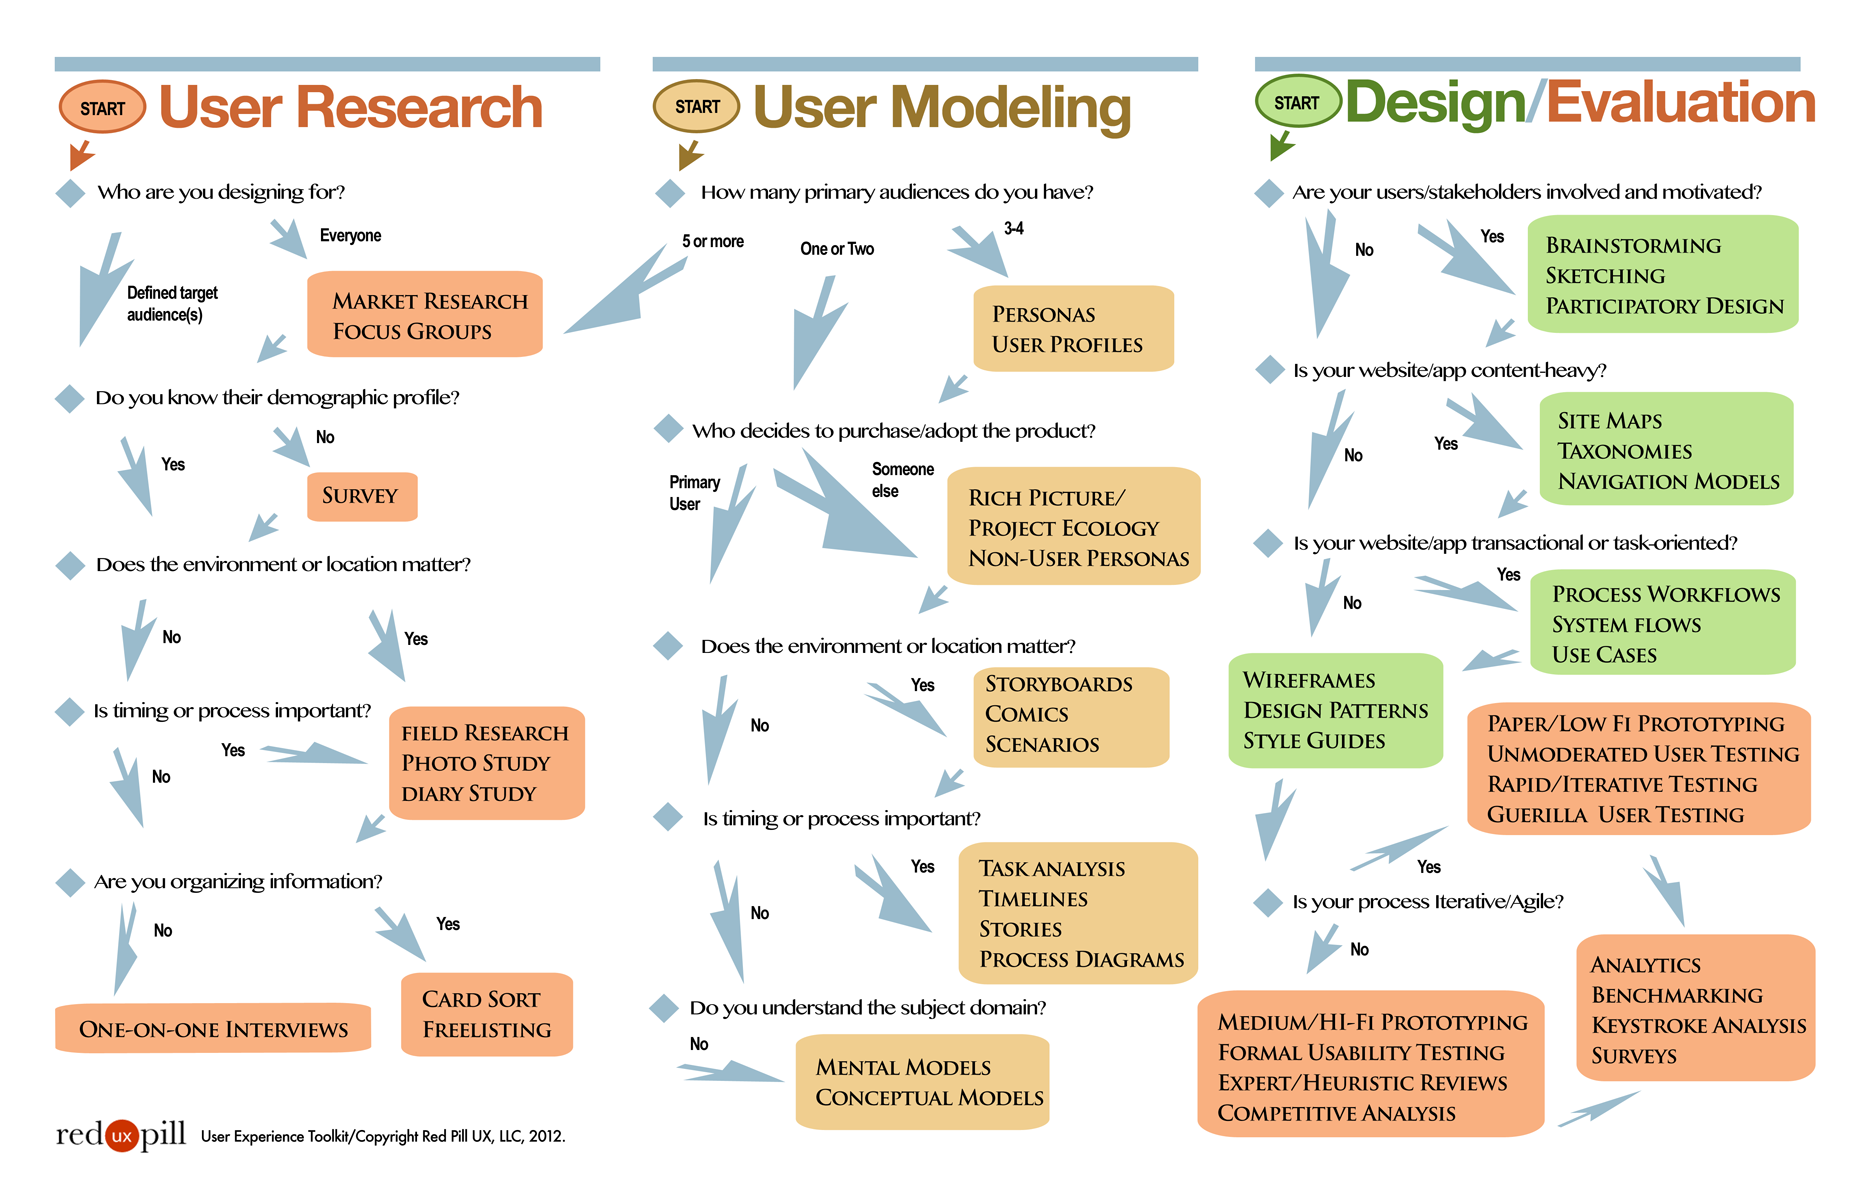
\includegraphics[width=16cm]{Img/CPD/3-FLOW.png}
\centering
\caption{\textbf{ \footnotesize{Diagrama de desición de investigación del usuario}}}
\label{fig:diagrama-desicion}
\end{figure}



\subsection{Declaración del problema}



\subsection{Suposiciones}
Las suposiciones son una declaración de alto nivel que pensamos que es cierta.

Todos los proyectos comienzan de este modo pero, normalmente, no hacen explícitas sus suposiciones. En lugar de ello, se ignoran o, en el peor de los casos, se tratan como si fueran hechos probados. En este trabajo se hace hincapié en las \textit{suposiciones de usuarios}, ya que las \textit{suposiciones de negocio} o mercado no intervienen en el desarrollo. A continuación una serie preguntas que resultan en suposiciones.


\begin{enumerate}

\item\textbf{¿Quiénes son los usuarios?}
\label{section.usuarios}
\begin{enumerate}
\item \textbf{Profesionales encargados de crear diseños 3D}. \vskip
Posee las capacidades técnicas y la experiencia sobre procesos y metodologías para llevar a cabo un proyecto de diseño en conjunto con el cliente/usuario.
\item \textbf{Personas sin conocimientos específicos}.\vskip
Desean participar del proceso de diseño pero sin tener conocimientos sobre diseño 3D. Interesados en encargar modelos 3D para la visualización o productos para la fabricación digital. Estas personas pueden ser emprendedores, artistas.
\item \textbf{Personas anónimas}.\vskip
Pueden visualizar los modelos 3D pero no participan en los procesos de diseño.
\end{enumerate}

\item{\textbf{¿Cómo encajaría el producto en su trabajo?}}

\begin{enumerate}

\item Sería excelente poder visualizar el producto en la web.

\item De manera positiva aunque un poco arriesgada por el cambio de paradigma.

\item Provocaría rechazo por personas con poca organización.

\item Positivo, sería muy interesante ver la organización de los diseños y el proceso.\vskip

\item Sería muy positivo si permite no depender tanto del email.\vskip

\end{enumerate}

\item{\textbf{¿Qué problemas soluciona el producto?}}

    \begin{enumerate}
    
    \item La visualización de un modelo 3D en proceso. \vskip
    
    \item Soluciona el diseño completo para personas que no saben de modelado 3D. \vskip
    
    \item La comunicación para discutir sobre un producto.\vskip
    
    \item La organización de los modelos y el progreso.\vskip
    
    \item Llevar un registro sobre los pagos y entregas.\vskip
    
    \end{enumerate}


\item{\textbf{¿Cuándo y cómo se utilizaría el producto?}}
    \begin{enumerate}
    \item En cualquier momento y en cualquier lugar, desde cualquier dispositivo con internet. \vskip
    
    \item En el lugar de trabajo en una intranet, así nadie puede ver los diseños.\vskip
    
    \item En cualquier momento y desde un dispositivo moderno.\vskip
    
    \item Sólo se utilizaría cuando se esté de viaje.\vskip
    
    \item Sólo desde la PC, sino es muy incómodo ver algo.\vskip
    
    \end{enumerate}


\item{\textbf{¿Cuáles serían las funciones más importantes?}}

    \begin{enumerate}
    \item Poder ver un modelo con muchos detalles, girarlo, agrandarlo, etc. \vskip
    
    \item Poder hacer cambios drásticos en los modelos sin necesidad de saber de 3D.\vskip
    
    \item Poder registrar los pagos para que haya transparencia.\vskip
    
    \item Poder comunicarse con el Diseñador y hacer feedback en una especie de chat.\vskip
    
    \item Poder hacer anotaciones en los modelos par que la otra persona vea. \vskip
    
    \item Tener registro de los pedidos de cambio con fecha y hora.\vskip
    
    \item Poder ver la evolución de los diseños y el tiempo que se tarda.\vskip
    
    \item Poder agregar documentos como planos, contratos.\vskip
    
    \item Poder ver como interactúa el producto con su entorno, por ejemplo en un paisaje o en un diseño de interiores.\vskip
    
    \item Poder ver con realidad virtual, con efectos realistas de movimientos.\vskip
    
    \end{enumerate}

\item{\textbf{¿Qué aspectos debe tener y cómo debe comportarse?}}

    \begin{enumerate}
    \item Debe ser bonito y fácil de usar. \vskip
    
    \item Debe ser parecido a los programas de CAD con mucha opciones y muy rápido.\vskip
    
    \item No importa si es bonito, lo importante es que funcione bien y rápido.\vskip

    \item Debe ser agradable a la vista y fácil de usar como una red social.\vskip
    \end{enumerate}

\end{enumerate}

\subsubsection{Priorización de las suposiciones} 
La razón por la que se declaran suposiciones al inicio del trabajo es poder identificar los riesgos del proyecto. Una vez que dispongamos de una lista de suposiciones se necesita averiguar cuáles de ellas tienen más riesgo. Lean UX lleva a cabo un ejercicio implacable de priorización. Una vez que se comprende que no se pueden probar todas las suposiciones del proyecto, la cuestión que se presenta es: ¿cuál de ellas se debe de probar primero? Para decidir sobre esta cuestión,  se puede crear un gráfico como el que aparece en la Figura \ref{fig:priori} y situar en él la lista de suposiciones. El objetivo del gráfico es decidir qué suposiciones se debe probar primero, en base en primer lugar, en su nivel de riesgo (por ejemplo, si se hiciera esto mal, ¿hasta qué punto se vería perjudicado el proyecto?) y, en segundo lugar, en el conocimiento que se tenga de la suposición. Cuánto más alto sea el riesgo que implica una suposición y menos se sepa de ella, mayor debe ser la prioridad. La asignación de la prioridad para la prueba no significa, ni mucho menos, que aquellas que no sean prioritarias desaparezcan del proyecto para siempre. Es recomendable mantener una lista de cuestiones pendientes con las suposiciones que no se hayan priorizado para poder volver a ellas y probarlas si se demuestra que amerita hacerlo.


\begin{figure}[h]
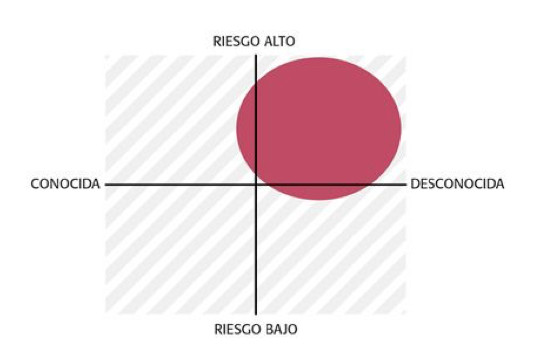
\includegraphics[width=8cm]{Img/UX/lean-supo.jpg}
\centering
\caption{\textbf{ \footnotesize{ Matriz de priorización }}}
\label{fig:priori}
\end{figure}


\subsection{Hipótesis}
Una vez se tenga la lista de suposiciones priorizada, se podrá dar el siguiente paso: probarlas. Para hacerlo, no obstante, será necesario transformar cada declaración de suposición a un formato más fácil de probar: Una descripción general de lo que se debe hacer y que impacto se espera. 

\subsubsection{Subhipótesis: división de las hipótesis en partes más pequeñas }\vskip
La hipótesis planteada es demasiado extensa la mayoría de las veces para que, con una única prueba, pueda determinarse su validez. Esto se produce porque la hipótesis contiene demasiadas partes móviles, es decir, demasiadas subhipótesis. Cuando esto sucede, se recomienda dividir las hipótesis en partes más pequeñas y específicas. Existen muchas maneras de hacerlo, pero para el trabajo de desarrollo de productos en particular creo que lo mejor es el siguiente formato: \vskip
\textit{Creemos que [haciendo esto - desarrollando esta función - creando esta experiencia de usuario] para [estas - personas - personajes] conseguiremos [este resultado].} 
Se sabrá si esto es correcto cuando se obtenga \textit{[este feedback del mercado, esta medida cuantitativa, o este conocimiento cualitativo]}\vskip El primer campo se completará con la función o mejora que está considerando para el producto. El segundo describirá exactamente qué clientes objetivo se beneficiarán de la función. El último campo, por su parte, especifica los beneficios que esos clientes obtendrán de ella. La frase final lo une todo. Esta frase determina si la hipótesis es cierta o no. ¿Qué resultado del feedback del mercado será el que indique que la idea es correcta? Podría ser una medida cuantitativa, como el uso que hacen los usuarios de una determinada función del producto, por ejemplo, o como el incremento de una métrica de negocio, o bien una medida cualitativa de alguna clase.




Desarrollar un software de comunicación eficiente en la revisión de diseños para un equipo multidisciplinario
logrará una mayor tasa de participación y un aumento en la satisfacción de los involucrados.
Se verificará que esto es cierto cuando aumenten las opiniones de los involucrados y se pueda registrar la evolución del diseño.


\subsection{Proto-personas}

Se usan Modelos de personas como arquetipos de usuarios que a su vez comparten características de determinados grupos de clientes o usuarios.
Son simplificaciones de personas para generar la conjetura más aproximada de quién utiliza el software y por qué. 

\begin{figure}[h]
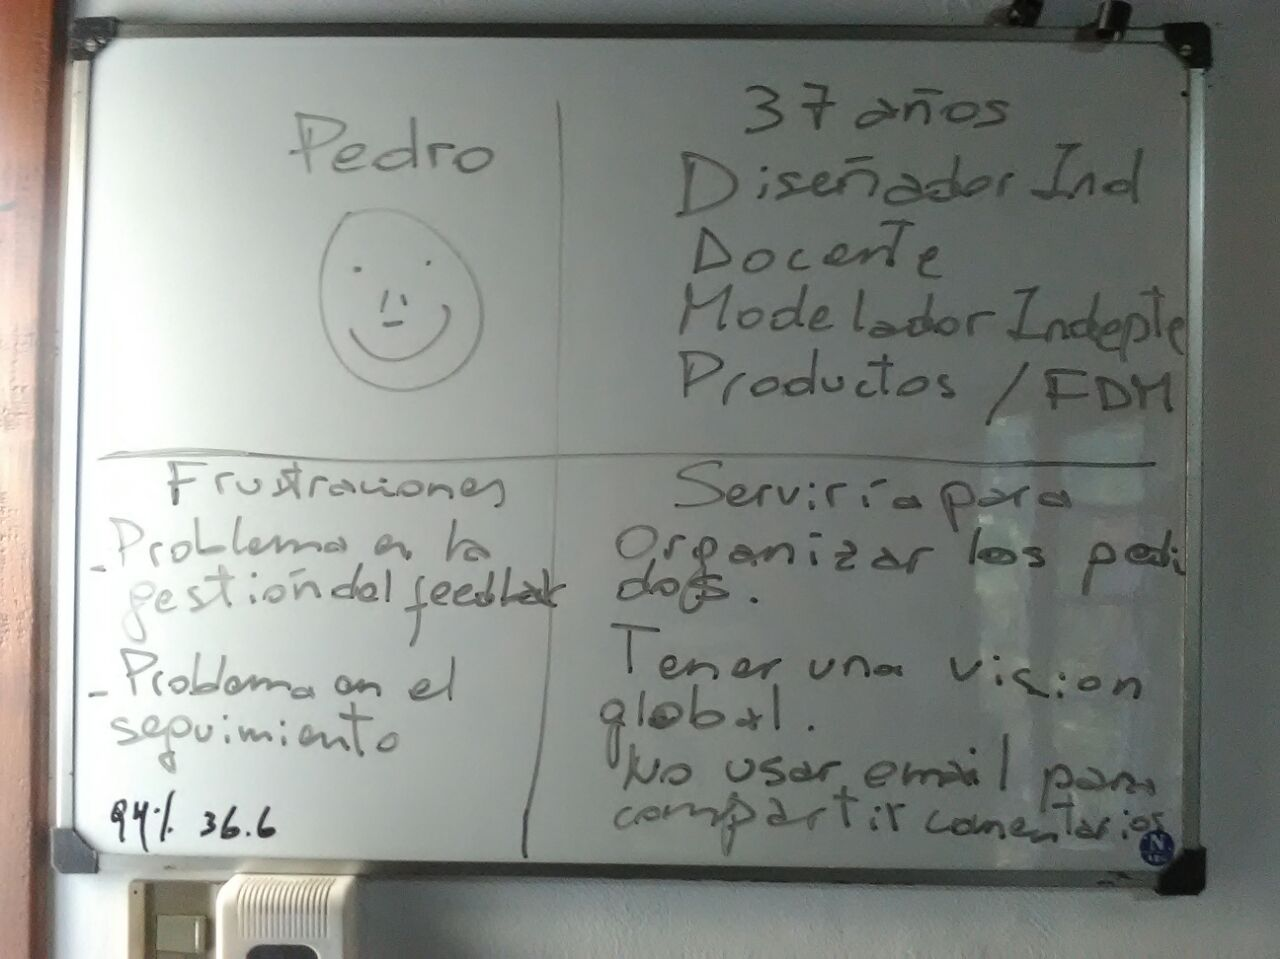
\includegraphics[width=10cm]{Img/UX/UX-proto.jpg}
\centering
\caption{\textbf{ \footnotesize{Proto-persona del profesional}}}
\end{figure}


\subsection{Funciones}
 Son las características, productos y los servicios que se pueden proponer para alcanzar esos resultados que necesita el usuario. El proceso de diseño luego comienza cuando se tiene noción de alguna característica y se trabaja para justificar la característica. En Lean UX, las características existen exclusivamente para satisfacer las necesidades del usuario.

\subsubsection{Sub-hipótesis con funciones: Historias}



\begin{tabular}{ |p{1cm}|p{3.5cm}|p{4.5cm}|p{4.5cm}| }

\hline
    Núm. & Se desarrolla & Para  & Para\\
\hline
1 & Un visualizador de modelos 3D & Para la persona con rol diseñador experto (XXX) & que solucione la visualización online de los avances de su trabajo \\
\hline
2 & Un visualizador de modelos 3D & Para la persona con rol diseñador experto (XXX) & que solucione la visualización online de los avances de su trabajo \\
\hline
\end{tabular}

- Ingreso / Modificación de parámetros
- Visor de historias / notas / chat
- Almacenamiento de archivos relacionados



\clearpage
\section{Diseño del prototipo}
Lean UX es un proceso colaborativo, un proceso que reúne a diseñadores y no diseñadores en un trabajo de creación conjunta. El diseño colaborativo es un enfoque que permite a los integrantes del equipo crear juntos los conceptos del producto. También les ayuda a construir un entendimiento común sobre el problema y sobre las soluciones de diseño. Asimismo, les permite decidir qué funcionalidad y elementos de la interfaz implementan mejor las funciones recogidas en sus hipótesis. La documentación de salida de estas sesiones consta normalmente de esquemas de baja fidelidad y \textit{wireframes}. Es básico que la documentación no esté muy elaborada para que el trabajo continúe siendo maleable. De esta manera, el equipo puede cambiar de dirección con facilidad una vez que sus pruebas les demuestren que el enfoque adoptado no funciona.

\subsection{Estudio de diseño}
El equipo re reune en una sesión más formal de trabajo o \textbf{Estudio de Diseño} (a veces también llamado Charrette de diseño)\citep{Gothelf2013} es una manera de conseguir que un equipo multidisciplinario visualice de forma conjunta las soluciones potenciales a un problema de diseño. Se usan técnicas específicas para llevar a cabo las sesiones de Estudio de Diseño y pueden organizarse de una forma más o menos formal, dependiendo de la situación del proyecto y los plazos de entrega. Abarca los siguientes pasos:
\begin{itemize}
    \item Definición del problema y sus restricciones. 
    \item Generación de ideas individuales (divergir). 
    \item Presentación y críticas. 
    \item Iteración y perfeccionamiento (emerger). 
    \item Generación de ideas del equipo (converger).
\end{itemize}


\begin{figure}[h]
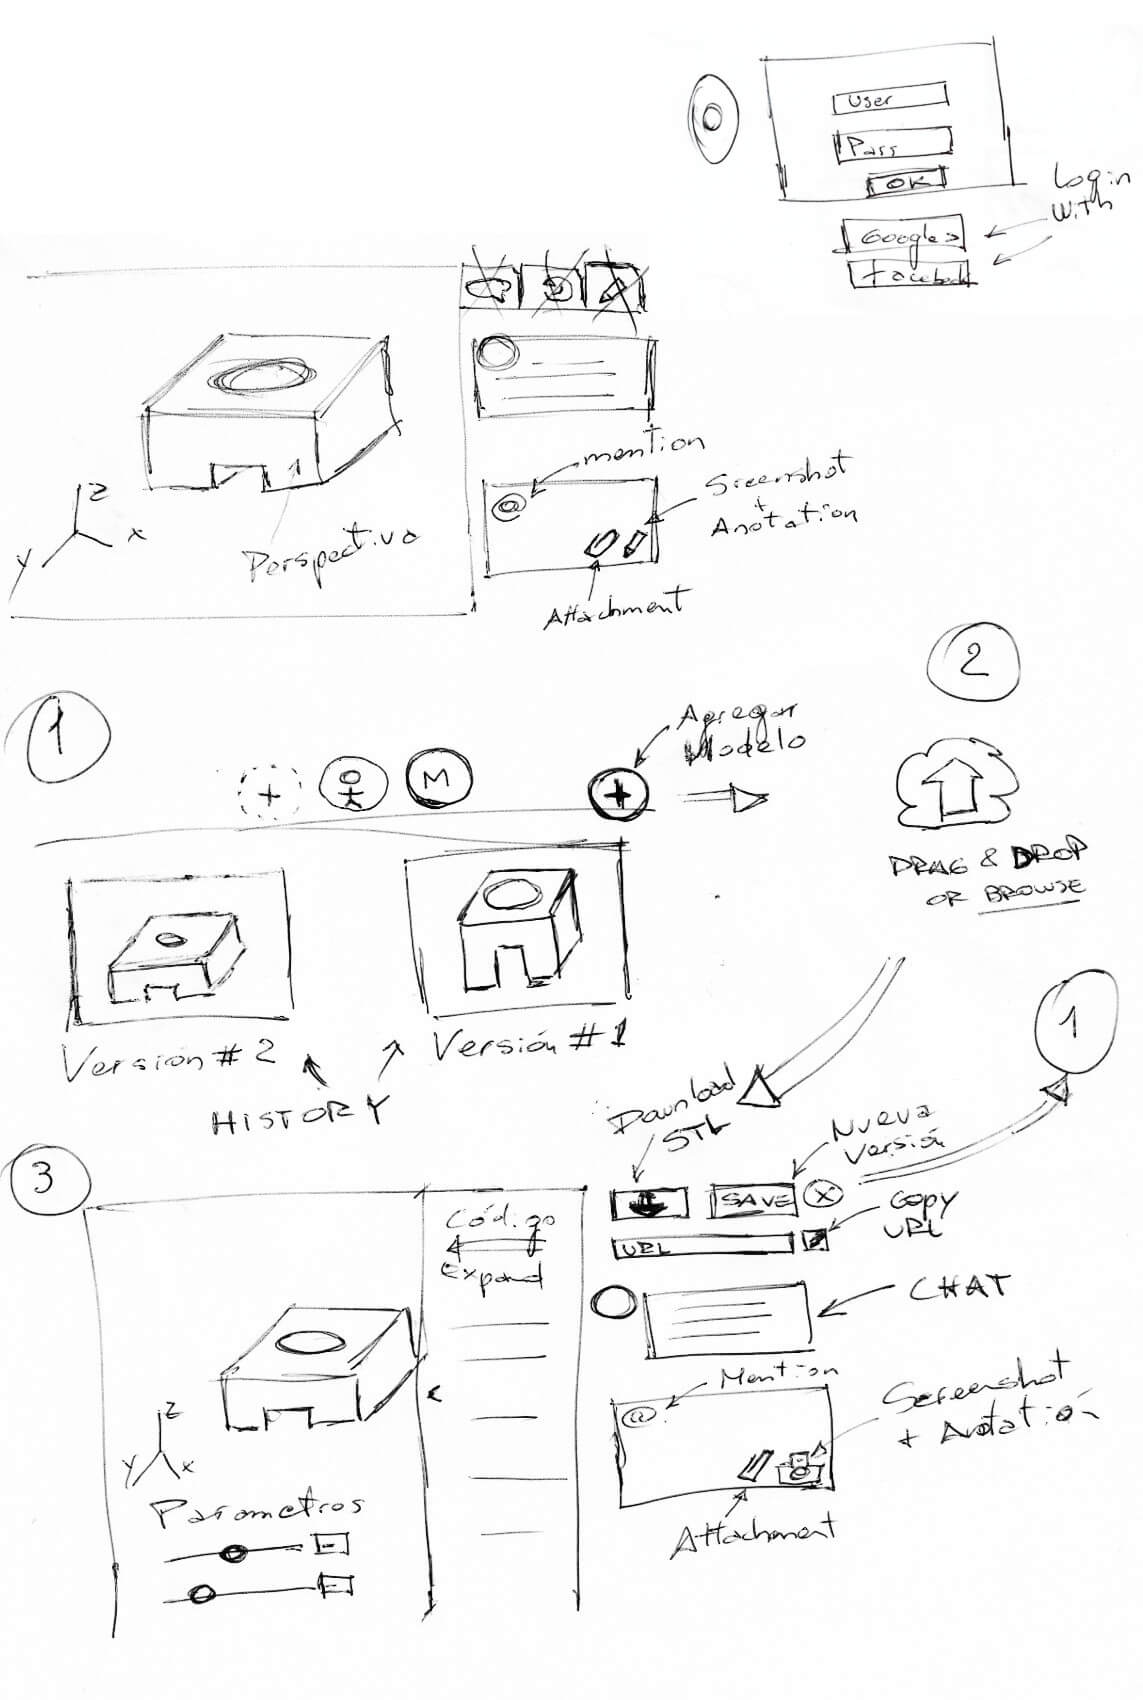
\includegraphics[width=14cm]{Img/UX/edc.jpg}
\centering
\caption{\textbf{ \footnotesize{Interfaz como salida del estudio de diseño}}}
\end{figure}


\begin{figure}[h]
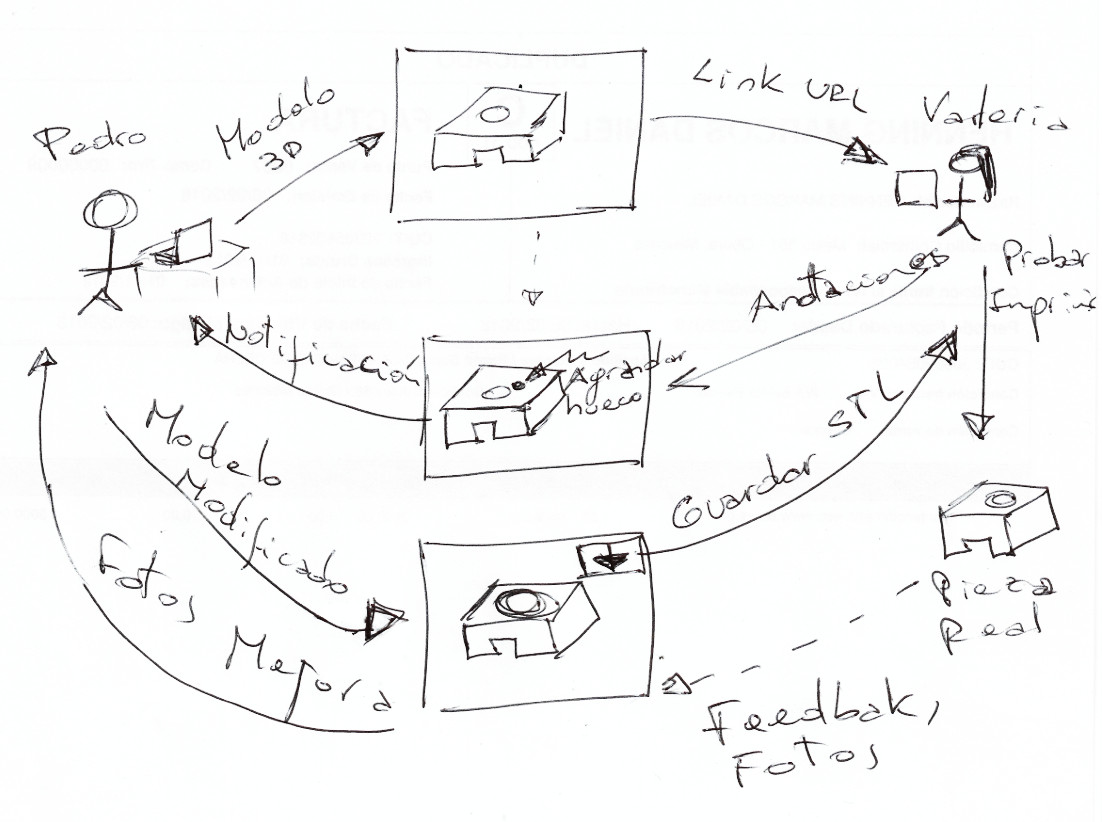
\includegraphics[width=14cm]{Img/UX/ed2.jpg}
\centering
\caption{\textbf{ \footnotesize{Posibles escenarios diseñados en el estudio de diseño}}}
\end{figure}

Los resultados del estudio de diseño se realizan comúnmente utilizando Lápices, Bolígrafos, Marcadores (de varios colores). Plantillas para esquemas, Pegatinas.

El objetivo del estudio del diseño es preparar todo el material para el siguiente paso de Lean UX: \textit{crear un PMV y probarlo con un experimento}.


\clearpage
\subsection{Definición de Componentes y Guías de estilo}
Una herramienta que facilita el diseño colaborativo es la guía de estilo, que es una biblioteca de patrones, ampliamente aceptada por todos, que codifica los elementos de texto, los gráficos y los interactivos de una interfaz de usuario y de un sistema. Estas guías (también conocidas como bibliotecas de patrones) son recopilaciones dinámicas de todos los componentes del producto a los que se enfrentará el usuario. Todo lo que forme parte de la experiencia del usuario aparece en la guía de estilo. Algunas empresas utilizan \textit{wikis} para las guías de estilo, lo que permite que toda la colección permanezca actualizada y que esté disponible para el equipo. Otros equipos, en cambio, prefieren crear guías de estilo ``dinámicas", es decir, repositorios de diseño y de código front-end\footnote{Front-end es la parte del software que interactúa con los usuarios.} que no solo definen el aspecto y el comportamiento del producto, sino que también proporcionan el lenguaje necesario y las hojas de estilo para la interfaz de cliente. De esta manera, al modificar la guía de estilo también se modifica el producto.
Para la estética del prototipo se eligió el concepto de diseño \textit{Material Design}\footnote{\url{https://material.io/guidelines/}}, un diseño donde la profundidad, las superficies, los bordes, las sombras y los colores juegan un papel principal. A continuación se especifican algunos componentes gráficos y diseños a utilizar:


\subsubsection{1. Tamaños de letras según dispositivos}
    \begin{figure}[h]
    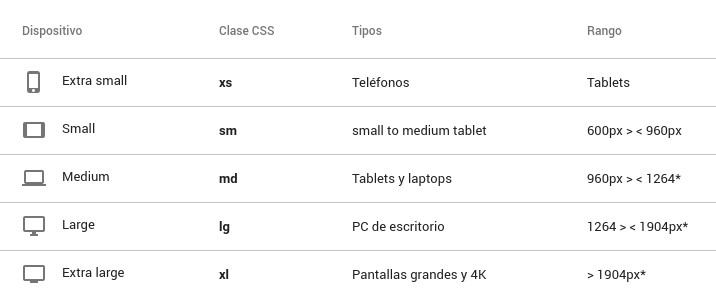
\includegraphics[width=14cm]{Img/UX/guia1.jpg}
    \centering
    \caption{\textbf{ \footnotesize{Tamaño de letras con sus respectivas clases CSS}}}
\end{figure} 
    
\subsubsection{2. Esquema de colores}
\begin{figure}[h]
    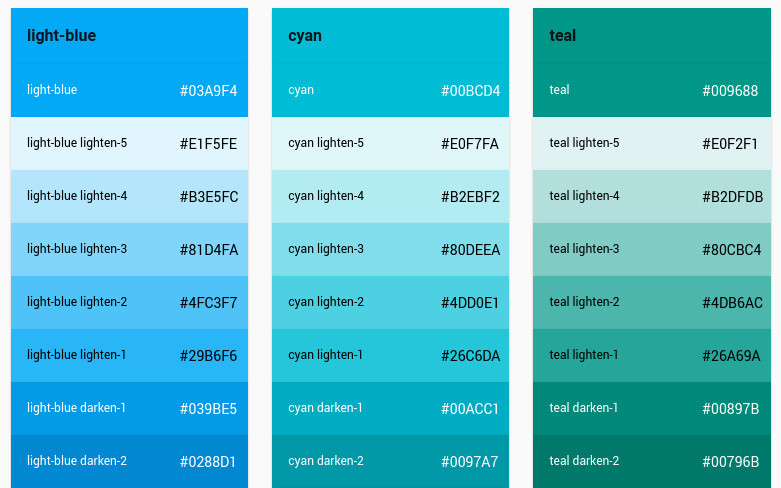
\includegraphics[width=12cm]{Img/UX/guia0.jpg}
    \centering
    \caption{\textbf{ \footnotesize{Esquema de colores con sus respectivas clases de CSS}}}
\end{figure}


\subsubsection{3. Iconos mediante fuentes tipográficas}
    Usando el prefijo fa- seguido del nombre del ícono como clase CSS. Las fuentes tipográficas son vectoriales, por lo que se puede cambiar el tamaño y color de los iconos sin perder calidad.
    \begin{figure}[h]
    
\includegraphics[width=11cm]{Img/UX/guia3.jpg}
    \centering
    \caption{\textbf{ \footnotesize{Iconos mediante fuentes tipográficas. Clase de CSS ej: .fa-email}}}
   
    \end{figure}
    
 
\subsubsection{4. Botones de acción simples}
    \begin{figure}[h]
    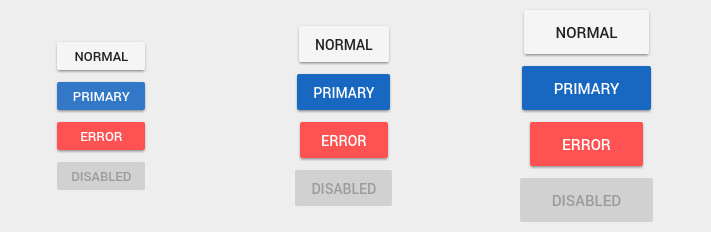
\includegraphics[width=11cm]{Img/UX/guia2.jpg}
    \centering
    \caption{\textbf{ \footnotesize{Estilos de botones. Clase de CSS ej: .btn.primary}}}
    \end{figure}
    
\clearpage
\subsubsection{5. Botones de acción flotante}\vskip
El Botón de Acción Flotante (FAB) es un botón circular con un ícono flotando en una página. El propósito de un FAB es parecido a un botón llamado-a-la-acción en ingles \textit{call-to-action}\footnote{\url{https://en.wikipedia.org/wiki/Call_to_action_(marketing)}}; enfatiza una acción que la mayoría de los usuarios presumiblemente realizaría. Generalmente se presenta con un color vívido que lo hace más prominente entre el resto de los elementos de la aplicación.
    \begin{figure}[h]
    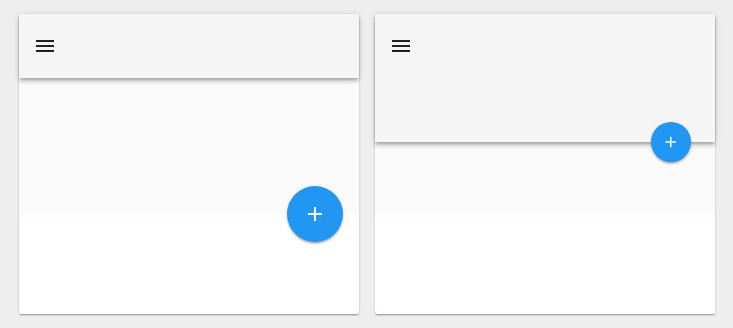
\includegraphics[width=12cm]{Img/UX/guia4.jpg}
    \centering
    \caption{\textbf{ \footnotesize{Botones de acción flotantes. Clase de CSS ej: .btn-floating.blue}}}
    \end{figure}
    

\subsubsection{6. Controles de entrada}\vskip
Estos elementos sirven para ser usados de múltiples formas. En el prototipo se utilizan sobre todo para la manipulación de parámetros de los modelos 3D y  también para la mayoría de los formularios.
    \begin{figure}[h]
    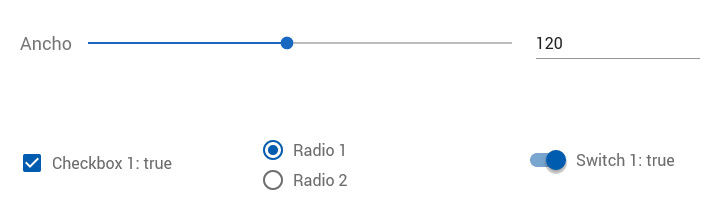
\includegraphics[width=14cm]{Img/UX/guia6.jpg}
    \centering
    \caption{\textbf{ \footnotesize{Controles gráficos.}}}
    \end{figure}



\clearpage  
\subsubsection{7. Cards o Tarjetas}\vskip
Las Tarjetas se están convirtiendo rápidamente en un patrón de UI indispensable, particularmente para las webs móviles. Esto se debe en parte a las webs como Pinterest\footnote{\url{https://pinterest.com}} y Twitter que hacen uso exhaustivo de las mismas. En el prototipo se utilizan tarjetas para listados o grillas de modelos que son parte de un proyecto.
    \begin{figure}[h]
    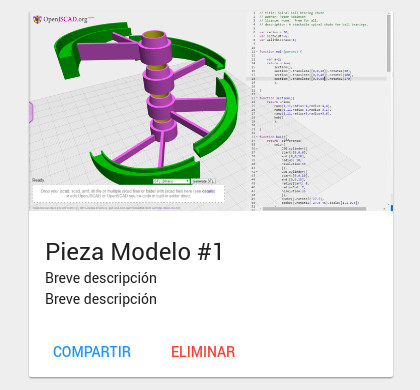
\includegraphics[width=7cm]{Img/UX/guia5.jpg}
    \centering
    \caption{\textbf{ \footnotesize{Tarjeta de un modelo 3D}}}
    \end{figure}
    
\subsubsection{8. Comentarios}\vskip
En el prototipo, los comentarios se pueden considerar tarjetas con un formato específico. Sirven para definir listados de comentarios o hilos de conversaciones, que hacen posible la comunicación entre los participantes de un proceso de diseño. Se pueden apreciar en la Figura \ref{fig:comment} el uso de hashtag (\#) y menciones (@), como en la mayoría de las redes sociales.
    \begin{figure}[h]
    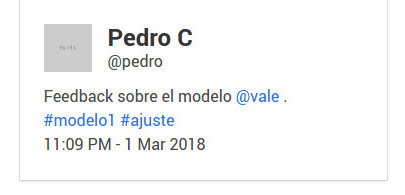
\includegraphics[width=7cm]{Img/UX/guia7.jpg}
    \centering
    \caption{\textbf{ \footnotesize{Tarjeta de comentario sobre un modelo.}}}
     \label{fig:comment}
    \end{figure}
    
    



\clearpage
\section{Producto Mínimo Viable}
Con las diferentes partes de las hipótesis definidas, se pueden determinar qué ideas sobre el producto son válidas y cuáles deben descartarse. El Producto Mínimo Viable (PMV) en inglés \textit{Minimum Viable Product} es importante porque probadas cuanto antes se encuentren las funciones en las que merece la pena invertir, antes se pueden centrar los recursos en las mejores soluciones. Este es uno de los modos principales que tiene Lean UX de minimizar el despilfarro. Se inicia con la lista de hipótesis priorizada. Para determinar la validez de las declaraciones de hipótesis se crean los mínimos elementos posibles. Esos elementos se son los \textbf{PMV}. Se utilizan luego para hacer experimentos. El resultado de esos experimentos indicará si la hipótesis fué correcta y si la dirección en la que se estaba trabajando es la indicada, debe perfeccionarse o debe abandonarse.

\subsection{Creación de un PMV}
Al comenzar la planificación de un PMV, lo primero que hay que tener en cuenta es lo que se quiere aprender con él. Por ello, resulta útil pensar estas tres cuestiones básicas: 
\begin{itemize}
    \item ¿Existe una necesidad para la solución que se diseña? 
    \item ¿Existe valor en la solución y las funciones que se ofrecen?
    \item  ¿La solución es usable?
\end{itemize}

Independientemente del propósito del PMV, esta etapa permite lanzar un producto y observar cómo interaccionan los usuarios con él en contextos realistas. Si con el PMV lo que se pretende es maximizar el aprendizaje, se debe:
\begin{itemize}
    \item Ser claro y conciso: dedicar el tiempo a depurar la idea hasta llegar a su proposición central de valor y presentar esa proposición a los usuarios. 
    \item Priorizar sin compasión: las ideas, como los artefactos, son pasajeras. Dejar que las mejores prueben su valor demostrando que aguantan el proceso de priorización. 
    \item Ser ágil: la información llega rápidamente, por lo que hay que asegurarse de durante el trabajo se pueda realizar actualizaciones con facilidad. 
    \item Medir el comportamiento: construir un PMV que permitan observar y medir lo que la gente hace realmente, no lo que dicen que hacen. En el diseño de productos digitales, el comportamiento es mucho más importante que las opiniones. 
    \item Utilizar una llamada-a-la-acción: se sabrá que el usuario valora la solución cuando demuestren que la usan.
\end{itemize}

\subsubsection{Creación del prototipo}
Una de las maneras más efectivas de crear los PMV es mediante un prototipo de la experiencia. \textit{Un prototipo es una aproximación de la experiencia de usuario que permite simular cómo será el uso del producto o servicio en cuestión}. Para que esa simulación sea efectiva deberá ser clicable (o bien tocarse con el dedo, dependiendo de la interfaz de usuario).
Por otra parte, como hay que dedicar el mínimo esfuerzo posible a su desarrollo, será importante que se elija bien la herramienta para crearlo. La elección de una herramienta u otra para el prototipo depende de: 
\begin{itemize}
    \item \textbf{¿Quién interactuará con él?} El primer prototipo lo utilizará el usuario 1.b establecido en la sección \ref{section.usuarios}: la persona sin conocimientos de diseño 3D.
    \item \textbf{¿Qué se espera aprender de él?} Se espera aprender aspectos de funcionalidad y usabilidad de la UI para visualizar un modelo 3D.
    \item \textbf{¿Cuánto tiempo se tiene para realizarlo?} Se cuenta con poco tiempo. Aproximandamente 4 días
\end{itemize}
  
\textbf{Desición del prototipo según la fidelidad}\vskip

La fidelidad se refiere al nivel de realismo en un prototipo. Por ejemplo, un prototipo de baja fidelidad podría ser los sketchs o diseños dibujados en papel. Un prototipo de alta fidelidad podría ser un prototipo que se vea e interactúe como un sitio web real. Mientras más alta sea la fidelidad, más se aprenderás. Por ejemplo, aprenderá sobre qué colores funcionan mejor para atraer la atención y qué piensan los usuarios sobre el aspecto y la sensación de su producto.
Si ya se ha desarrollado la guía de estilo existente, entonces es más fácil usar alta fidelidad porque no hay que pensar en la mayoría de las decisiones estéticas y se puede enfocar hacia la funcionalidad. Para el prototipo se decide utilizar \textit{Prototipos de media y alta fidelidad} y \textit{Prototipos codificados} debido a que las decisiones de funcionalidad en primera instancia fueron discutidas con los sketches en el estudio de diseño, y el diseño estético se estableció en la guía de estilos.
A continuación se ilustra un gráfico de fidelidad en 2 dimensiones para la desición del tipo de prototipo.


 \begin{figure}[h]
    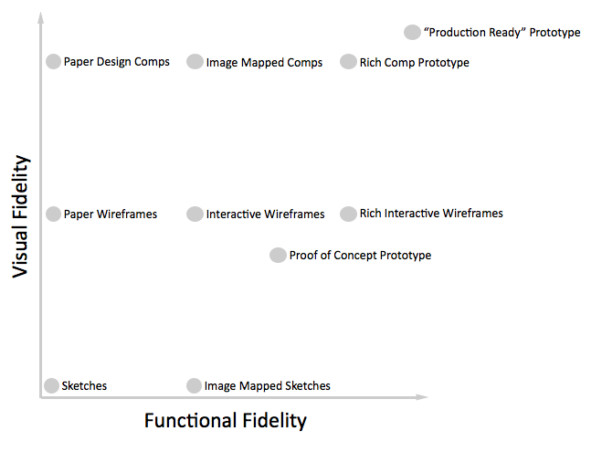
\includegraphics[width=12cm]{Img/UX/prototipo0.jpg}
    \centering
    \caption{\textbf{ \footnotesize{Elección de la herramienta}}}
     \label{fig:comment}
\end{figure}


Una vez elegida la herramienta para crear el PMV se inicia la construcción del prototipo, no es necesario incluir la experiencia de usuario completa del producto. En lugar de eso, se simula la parte más importante de esa experiencia. Se hace foco en los flujos de trabajo principales que ilustran el PMV. De esta manera el equipo puede observar una parte específica de la experiencia de usuario (tal y como será) para que puedan valorar su validez y su eficacia.

 \begin{figure}[h]
    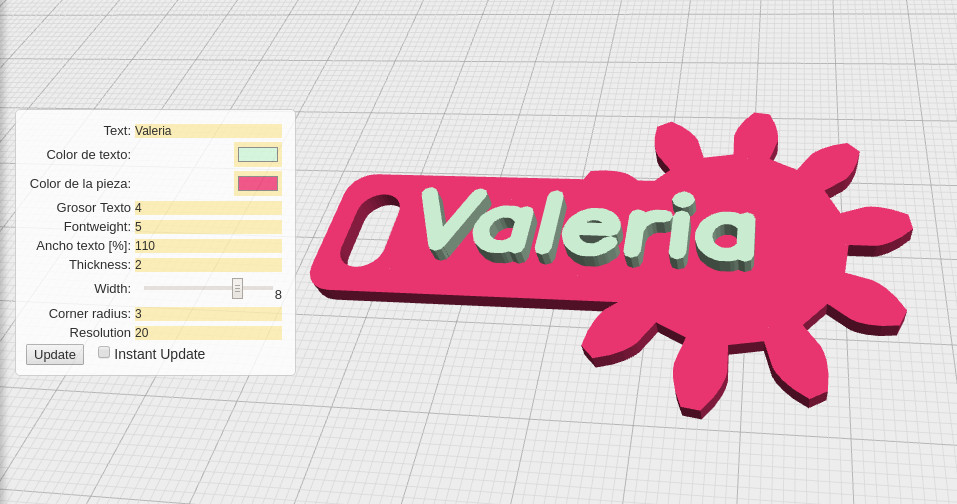
\includegraphics[width=12cm]{Img/UX/feedback0.jpg}
    \centering
    \caption{\textbf{ \footnotesize{Feedback}}}
     \label{fig:comment}
\end{figure}



\section{Diseño colaborativo}

\subsection{Mockup}

\subsection{One Page / Single-page application}
http://1.droppdf.com/files/A32RR/manning-single-page-web-applications-javascript-end-to-end-2014.pdf

(https://theseus.fi/bitstream/handle/10024/97217/Kokkonen_Juha.pdf?sequence=1 ,pag 9)

Las aplicaciones web de una sola página proporcionan una experiencia similar a las de escritorio en un navegador web estandar. 

\subsection{Programación Reactiva}
\subsection{Programación Reactiva (Manifiesto)}
(traducción en odt)
\begin{itemize}
\item Responsivo:
\item Resiliente:
\item Elástico:
\item Dirigido por Mensajes:
\end{itemize}
\subsection{Relación entre el patrón de diseño observable y la Programación Reactiva}
(en vuejs odt)
\subsection{--FrontEnd--}
\subsection{vue.js}
guia español: https://es-vuejs.github.io/vuejs.org/v2/guide/

rendimiento vue
https://www.kairosds.com/blog/vue-js-exito/

\subsection{Guías de estilo: Bulma}
\subsection{nuxt.js}

Traduciendo libremente la explicación que aparece en la página de nuxt.js:

    El 25 de octubre de 2016, el equipo detrás de zelt.co, anuncia Next.js, un framework para aplicaciones React renderizadas en el lado servidor. Pocas horas después de ese anuncio, la idea de crear aplicaciones renderizadas del lado servidor en Vue.js de la misma forma que Next.js era obvia. Nuxt.js había nacido.
https://www.opsou.com/es/blog/nuxtjs-una-pieza-mas-del-ecosistema-vuejs-introduccion


Nuxt.js es un framework para crear aplicaciones universales en Vue.js. Una aplicación universal es aquella que su código puede ser ejecutado tanto en el cliente como en el servidor. Nuxt.js tiene muchas características, pero una de las más interesantes es que nos ayuda a crear aplicaciones Vue.js que se renderizan del lado del servidor (SSR – Server-Side Rendering). Esto quiere decir que se precargan las páginas en el servidor y luego se envía el HTML renderizado al navegador.
https://www.groloop.com/vue-js-2-12-aplicaciones-vue-js-universales-con-nuxt-js/

Una aplicación universal es aquella que comparte todo (o casi todo) su código entre el cliente y el servidor.
https://medium.com/@sergiodxa/qu%C3%A9-es-una-aplicaci%C3%B3n-universal-f1258d030f25

ventajas y desventajas
https://github.com/i62navpm/Tutorial-Nuxt

\subsection{--Backend--}
\subsection{node.js}
\subsection{express}
\subsection{API RESTFUL}
ver PDF: API REST y sistema de aprovisionamiento en containers para servIoTicy

book: https://www.amazon.es/RESTful-API-Design-Practices-API-University-ebook/dp/B01L6STMVW

Tesis Doctoral: http://www.ics.uci.edu/~fielding/pubs/dissertation/rest_arch_style.htm
Artículo: https://www.infoq.com/articles/subbu-allamaraju-rest
Book: https://pages.apigee.com/rs/apigee/images/api-design-ebook-2012-03.pdf (ver fuentes)
Book: https://doc.lagout.org/programmation/Webservers/REST%20API%20Design%20Rulebook%20-%20Masse%20-%20O%27Reilly%20%282012%29/REST%20API%20Design%20Rulebook%20-%20Masse%20-%20O%27Reilly%20%282012%29.pdf

Consideraciones de diseño 
  - no verbos
  - url en minuscula, no usar _ 
  - usar uri
  
Metodos get/post/delete/etc

\subsection{ORM: sequelize}
http://docs.sequelizejs.com/

\subsection{--test--}
\subsection{¿Framework para test?}


\section{MVP - Prototipado}
\subsection{Prototipado rápido HTML más Bulma}

\begin{figure}
\centering
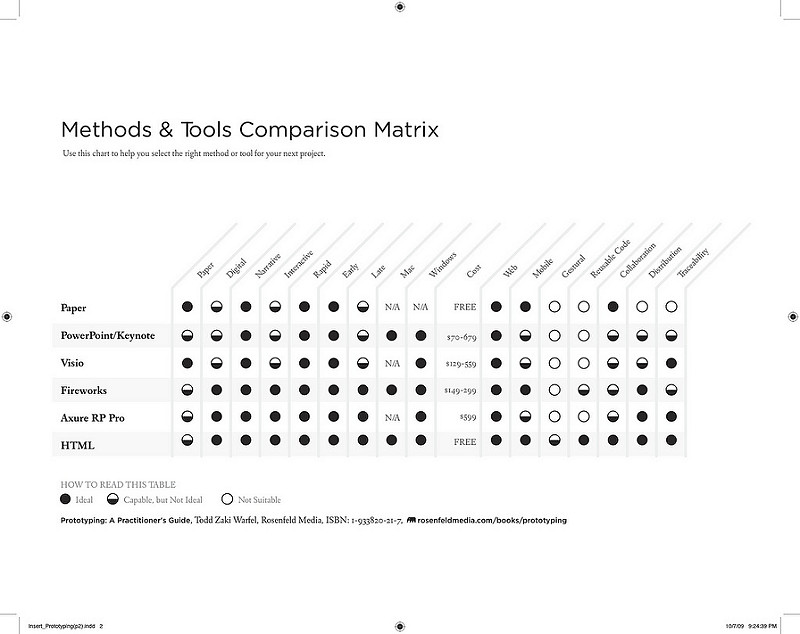
\includegraphics[width=16cm]{Img/UX/UX-matrix.jpg}
\caption[Proto-persona (optional short caption)]{\label{us_figure} Matriz de herramientas para prototipado. Extender a nuevas herramientas}
\end{figure}

\section{Herramientas tecnológicas para el desarrollo}

\subsection{Lenguaje Ubicuo: De Historias a Escenarios y tests}

Scenario: Listar los Trabajos\vskip0mm
  Given: Estoy en URL\vskip0mm
  Then: Veo el título "Pieza de Pruebas"\vskip10mm
 
Scenario: Acceder al Escritorio de Trabajo\vskip0mm
  Given: Estoy en URL\vskip0mm
  When: Hago click en "Pieza de Pruebas"\vskip0mm
  Then: Estoy en URL\vskip0mm
  Then: Veo el título "Pieza de Pruebas"\vskip0mm
  And: Veo la etiqueta "Alto"\vskip0mm
  And: Veo la etiqueta "Ancho"\vskip0mm
  And: Veo la etiqueta "Profundidad"\vskip0mm
  And: Veo el Visor de la Pieza "stl-view"
  
\subsection{Especificación BDD Escenarios, Cucumber, etc}

\subsection{Programación SPA (Single Page App)}

\begin{displayquote}
An SPA is an application delivered to the browser that doesn’t reload the page during use. Like all applications, it’s intended to help the user complete a task, such as “write a document” or “administer a web server.” We can think of an SPA as a fat client that’s loaded from a web server. \cite{Mikowski2015}
\end{displayquote}

\say{The single-page web interface is composed of individual components which can be updated/replaced independently, so that the entire page does not need to be reloaded on each user action.\cite{Mesbah2007}}


\subsection{Visualización y datos (WebGL, OpenJSCAD)}

\subsection{Frontend Vue.js}

\subsection{Backend (Node.js, Express, GraphQL, ES 2015 )}


\section{Métricas, ecuaciones, fórmulas, posibilidades}


\section{Construcción del sistema}

\subsection{Modelado de Classes}

\subsection{Diseño y Código en JS (FLUX?)}

\subsection{API: GraphQL}


\section{Funcionalidades}

\subsection{Control de versiones}

\subsection{Integración con otras plataformas (embed)}

\subsection{Compartir proyectos (share)}

\subsection{Exportar modelos}

\subsection{Extras: Anotaciones, comentarios, adjuntar imagen, chat, etc}
